% Chapter 2: Flow Chart
% Financial Reporting Processes and Workflows

\chapter{Flow Chart}

\section{Financial Reporting Process Flow}

\subsection{Monthly Reporting Cycle Overview}
The financial reporting process at Asia Trade \& Technology follows a structured monthly cycle that ensures timely and accurate financial information is collected, verified, and processed. This process is essential for maintaining financial control and ensuring that all project expenses are properly documented and approved before payment processing.

The monthly cycle begins with the collection of financial data from field accountants and continues through various stages of verification, approval, and final processing. Each stage has specific responsibilities and timelines that must be followed to maintain the integrity of the financial reporting system. The entire process is designed to ensure that all financial transactions are properly recorded, verified, and approved according to company policies and international accounting standards.

The monthly reporting cycle is synchronized with the company's fiscal calendar and is coordinated with the headquarters in Beijing to ensure consistency across all international operations. This synchronization helps to maintain accurate financial records and enables timely reporting to stakeholders and regulatory authorities.

\begin{figure}[H]
    \centering
    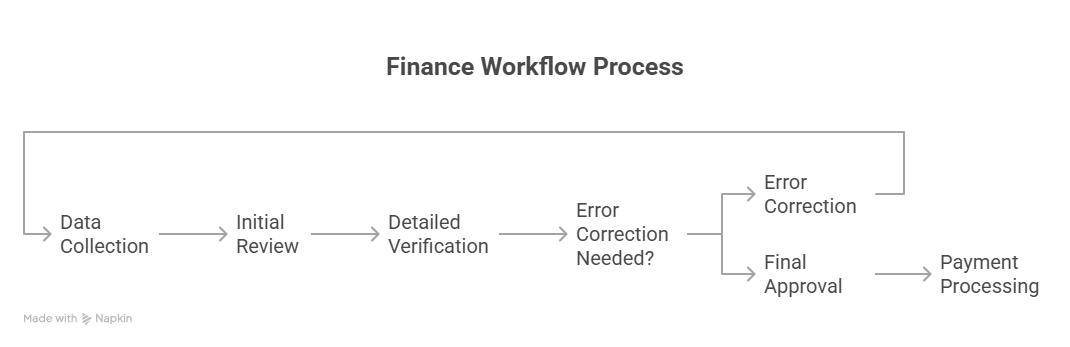
\includegraphics[width=0.9\textwidth]{assets/images/financial_flowchart.png}
    \caption{Monthly Financial Reporting Process Flow}
    \label{fig:financial_flowchart}
\end{figure}

Figure \ref{fig:financial_flowchart} illustrates the complete monthly financial reporting process flow, showing the sequential stages from data collection to final payment processing. The flowchart demonstrates the systematic approach used to ensure accuracy and compliance throughout the entire reporting cycle.

\subsection{Data Collection Phase}
The first phase of the financial reporting process involves the collection of financial data from various field locations. In the case of the River Protection project, financial reports are collected from the accountant working in the Brahmanbaria area. These reports include detailed information about all expenses incurred during the month, including materials, labor costs, equipment rentals, and other project-related expenses.

The field accountant is responsible for compiling all financial documents, including receipts, invoices, timesheets, and other supporting documentation. These documents are organized according to expense categories and submitted along with a summary report that outlines the total expenses for the month. The data collection phase typically takes place during the first week of each month, allowing sufficient time for compilation and initial review.

During the data collection phase, the field accountant must ensure that all expenses are properly categorized and that all supporting documentation is complete and accurate. This includes verifying that all receipts and invoices are properly signed and authorized, checking that expense amounts match the supporting documentation, and ensuring that all expenses fall within the approved budget categories.

\subsection{Initial Documentation Review}
Once the financial reports are received from the field accountant, the initial documentation review begins. This phase involves a thorough examination of all submitted documents to ensure completeness and basic accuracy. The review process includes checking that all required documents are present, verifying that expense amounts match the supporting documentation, and ensuring that all expenses are properly categorized.

During this phase, any obvious errors or missing documents are identified and flagged for correction. The review process also includes checking that all expenses fall within the approved budget categories and that proper authorization has been obtained for any expenses that exceed normal limits. This initial review helps to identify issues early in the process and reduces the need for corrections at later stages.

The initial documentation review is conducted by the accounting team in the Dhaka office, who have been trained to identify common errors and discrepancies. This review serves as the first line of defense against financial errors and helps to ensure that only accurate and complete reports proceed to the next stage of the process.

\subsection{Detailed Verification Process}
The detailed verification process is the most critical phase of the financial reporting cycle. During this phase, each expense item is carefully examined to ensure accuracy, completeness, and compliance with company policies and project requirements. The verification process includes several key checks that must be completed before the report can be approved.

The verification process includes checking that all receipt amounts match the reported expenses, verifying that all expenses are within the project budget, ensuring that proper authorization has been obtained for all purchases, and confirming that all expenses are legitimate project-related costs. Any discrepancies or issues identified during this phase must be resolved before the report can proceed to the next stage.

The detailed verification process is conducted by experienced accounting professionals who have been trained in international accounting standards and company policies. This process may involve cross-checking information with other departments, verifying authorization signatures, and confirming that all expenses are properly documented and justified.

\subsection{Error Correction and Resubmission}
When errors or missing documents are identified during the verification process, the report is returned to the field accountant for correction. The error correction process involves clearly communicating the issues that need to be addressed and providing guidance on how to resolve them. The field accountant is responsible for gathering any missing documents, correcting any calculation errors, and providing additional clarification where needed.

The resubmission process ensures that all corrections are properly documented and that the revised report includes all necessary supporting documentation. This iterative process continues until all issues are resolved and the report meets the required standards for accuracy and completeness. The error correction and resubmission phase is essential for maintaining the quality and reliability of the financial reporting system.

The error correction process is designed to be educational as well as corrective. Field accountants are provided with feedback and training to help them avoid similar errors in the future. This approach helps to improve the overall quality of financial reporting and reduces the need for corrections in subsequent reporting cycles.

\subsection{Final Approval and Processing}
Once the financial report has passed all verification checks and any necessary corrections have been made, it is ready for final approval. The final approval process involves a comprehensive review by the manager in the Dhaka office, who examines the entire report to ensure that all requirements have been met and that the financial information is accurate and complete.

After the manager's approval, the report is forwarded to the head office for payment processing. The payment processing phase involves the generation of payment vouchers, the preparation of payment documentation, and the coordination with the finance department to ensure that all approved expenses are paid in a timely manner. This final phase completes the monthly financial reporting cycle and ensures that all project expenses are properly accounted for and paid.

The final approval and processing phase also includes the preparation of summary reports for senior management and the updating of financial records and databases. This ensures that all financial information is properly recorded and available for future reference and analysis.

\section{Document Management System}

\subsection{Document Classification and Organization}
The document management system at Asia Trade \& Technology is designed to ensure that all financial documents are properly organized, stored, and easily accessible when needed. Documents are classified into different categories based on their type, purpose, and importance. This classification system helps to maintain order and facilitates quick retrieval of specific documents when required.

The main categories of documents include receipts, invoices, timesheets, purchase orders, authorization letters, and project reports. Each category has specific requirements for storage, retention, and access. Documents are also organized by project, date, and expense type to ensure that related documents can be easily located and reviewed together.

The document classification system is designed to be flexible and scalable, allowing for the addition of new categories as the company's operations expand. This system is regularly reviewed and updated to ensure that it continues to meet the needs of the organization and complies with changing regulatory requirements.

\begin{figure}[H]
    \centering
    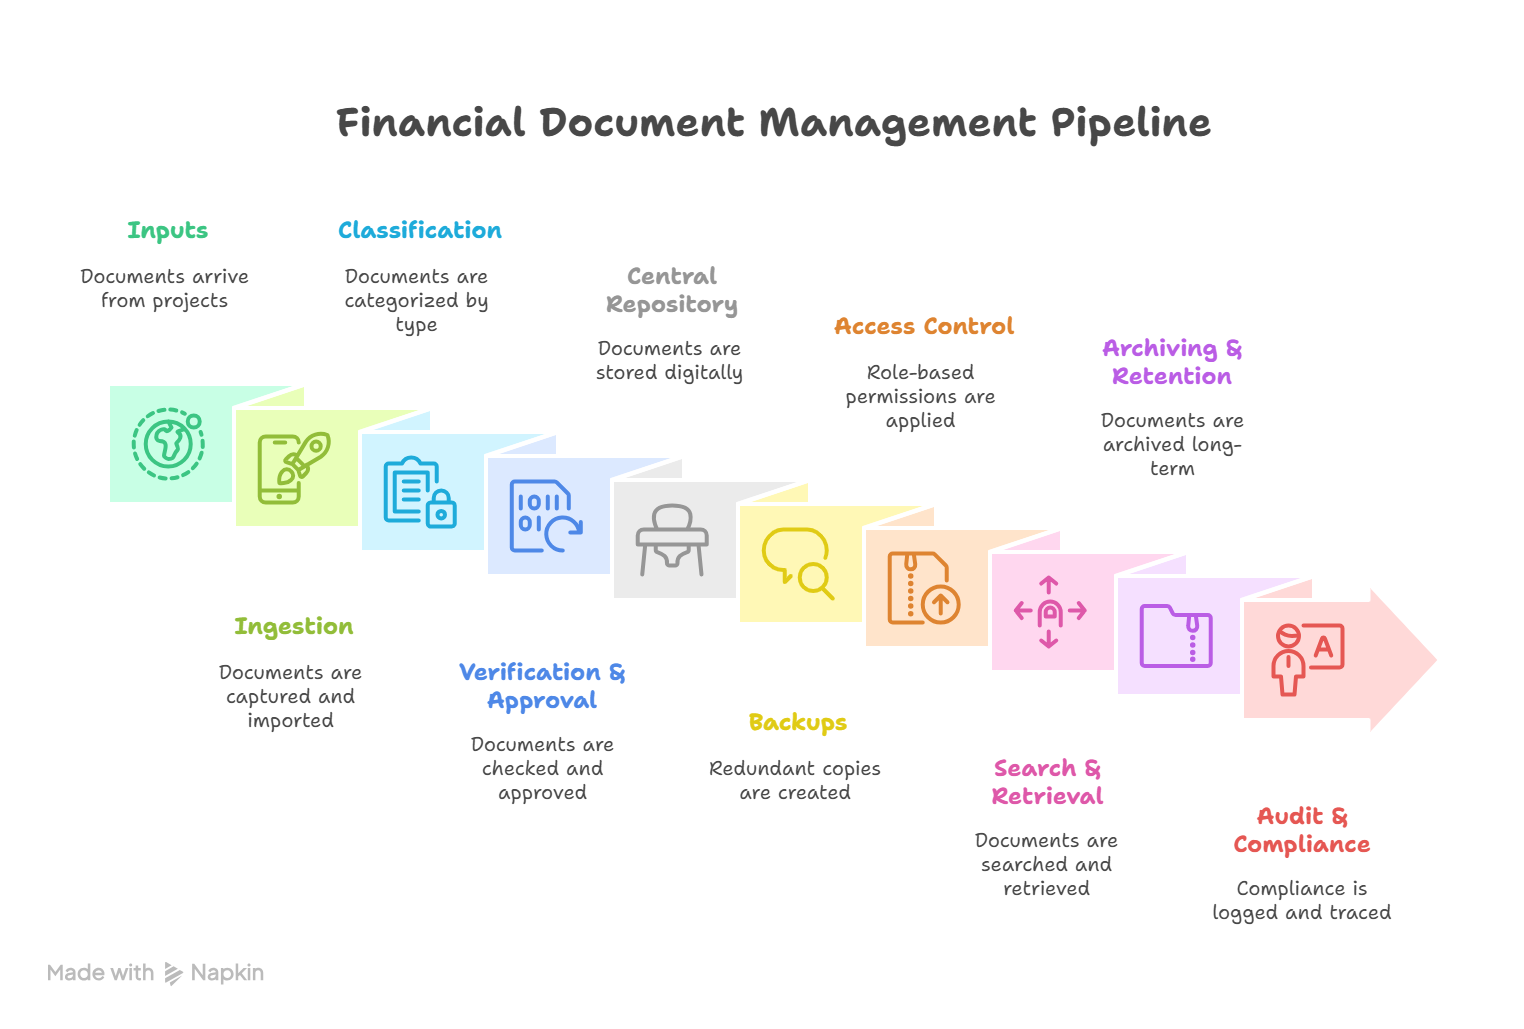
\includegraphics[width=0.9\textwidth]{assets/images/document_management.png}
    \caption{Document Management System Architecture}
    \label{fig:document_management}
\end{figure}

Figure \ref{fig:document_management} shows the comprehensive document management system architecture, illustrating the flow from document input through classification, verification, storage, and archiving. The diagram highlights the dual storage approach and security measures implemented to protect sensitive financial information.

\subsection{Receipt and Invoice Processing}
Receipts and invoices are the most important documents in the financial reporting process, as they provide proof of expenses and support the accuracy of financial reports. The processing of these documents involves several steps that ensure their validity and completeness. Each receipt and invoice is carefully examined to verify that it contains all required information, including the date, amount, description of goods or services, and vendor details.

The processing system includes checking that receipts and invoices are properly signed and authorized, verifying that amounts match the reported expenses, and ensuring that all supporting documentation is attached. Any discrepancies or missing information are flagged for correction before the documents are accepted into the system. This thorough processing helps to maintain the integrity of the financial records and prevents errors from being carried forward.

The receipt and invoice processing system is designed to be efficient and accurate, with multiple checkpoints to ensure that all documents are properly processed and recorded. This system helps to prevent fraud and errors while ensuring that all legitimate expenses are properly documented and approved.

\subsection{Document Verification Checklist}
A comprehensive verification checklist is used to ensure that all documents meet the required standards before they are accepted into the financial reporting system. This checklist includes items such as document completeness, accuracy of information, proper authorization, and compliance with company policies. Each document must pass all checklist items before it can be included in the financial report.

The verification checklist is designed to catch common errors and omissions that could affect the accuracy of financial reports. Items on the checklist include checking that all required fields are filled in, verifying that amounts are correctly calculated, ensuring that proper authorization has been obtained, and confirming that documents are properly dated and signed. This systematic approach helps to maintain consistency and quality in the document verification process.

The verification checklist is regularly updated to reflect changes in company policies, regulatory requirements, and best practices. This ensures that the checklist remains relevant and effective in maintaining the quality of financial documentation.

\subsection{Digital and Physical Storage Systems}
The company maintains both digital and physical storage systems for financial documents to ensure their security and accessibility. Digital storage systems are used for electronic documents and scanned copies of physical documents, while physical storage is maintained for original documents that require secure long-term storage. Both systems are designed to protect documents from damage, loss, or unauthorized access.

The digital storage system includes backup procedures and access controls that ensure documents are protected and available when needed. Physical storage systems include secure filing cabinets and storage rooms that are protected from environmental damage and unauthorized access. Regular audits are conducted to ensure that both storage systems are functioning properly and that documents are being stored according to established procedures.

The dual storage system provides redundancy and ensures that documents are protected against various types of risks, including natural disasters, technical failures, and unauthorized access. This approach helps to ensure the long-term preservation and accessibility of important financial documents.

\subsection{Document Retention and Archiving}
The company has established clear policies for document retention and archiving that ensure important documents are preserved for the required period while allowing for the disposal of outdated or unnecessary documents. Retention periods are determined based on legal requirements, business needs, and regulatory compliance. Different types of documents have different retention periods based on their importance and legal requirements.

The archiving process involves transferring documents from active storage to long-term storage when they are no longer needed for current operations. Archived documents are stored in a secure location and are accessible when needed for audits, legal proceedings, or historical reference. The archiving system includes proper indexing and cataloging to ensure that archived documents can be easily located when required.

The document retention and archiving system is designed to comply with international standards and local regulatory requirements. This system helps to ensure that the company maintains proper records while managing storage costs and maintaining efficient access to current documents.

\subsection{Access Control and Security}
Access to financial documents is controlled through a system of permissions and security measures that ensure only authorized personnel can view or modify documents. Access levels are determined based on job responsibilities and the need to know specific information. Regular reviews of access permissions are conducted to ensure that access rights remain appropriate and up to date.

Security measures include password protection for digital systems, physical security for storage areas, and audit trails that track who has accessed specific documents and when. These security measures help to protect sensitive financial information and ensure that documents are not compromised or accessed by unauthorized personnel. Regular security audits are conducted to identify and address any potential vulnerabilities in the system.

The access control and security system is designed to balance the need for accessibility with the requirement for security. This system ensures that authorized personnel can access the documents they need to perform their duties while protecting sensitive information from unauthorized access.

\section{Approval Hierarchy \& Workflow}

\subsection{Multi-Level Approval Structure}
The approval hierarchy at Asia Trade \& Technology follows a structured multi-level system that ensures proper oversight and control over financial decisions. This hierarchical structure is designed to prevent errors, ensure compliance with company policies, and maintain accountability at all levels of the organization. Each level of approval has specific responsibilities and authority limits that are clearly defined and communicated to all personnel.

The approval hierarchy typically includes three main levels: field-level approval, office-level approval, and headquarters-level approval. Each level serves a specific purpose in the approval process and helps to ensure that all financial decisions are properly reviewed and authorized before being implemented. This multi-level approach helps to distribute responsibility and reduce the risk of errors or unauthorized expenditures.

The multi-level approval structure is designed to be efficient while maintaining proper controls. Each level has specific authority limits and is responsible for reviewing decisions made at lower levels. This structure helps to ensure that all financial decisions are properly reviewed and authorized while maintaining efficient operations.

\begin{figure}[H]
    \centering
    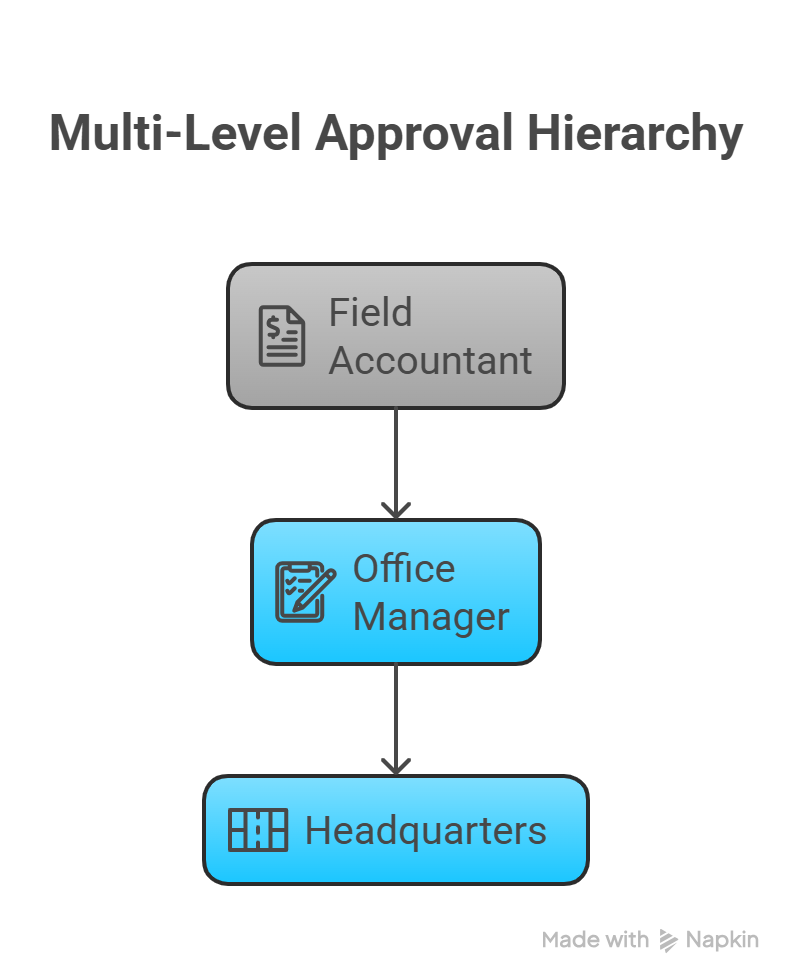
\includegraphics[width=0.9\textwidth]{assets/images/approval_hierarchy.png}
    \caption{Multi-Level Approval Hierarchy Structure}
    \label{fig:approval_hierarchy}
\end{figure}

Figure \ref{fig:approval_hierarchy} presents the organizational structure of the approval hierarchy, showing the three main levels of authority and their respective responsibilities. The diagram illustrates the flow of information and decision-making authority from the field level through regional management to headquarters, along with the communication channels that facilitate effective coordination.

\subsection{Field-Level Approval Process}
The field-level approval process is the first step in the approval hierarchy and involves the review and approval of expenses by personnel working directly at project sites. In the case of the River Protection project, the field accountant in the Brahmanbaria area is responsible for the initial review and approval of all local expenses. This includes verifying that expenses are legitimate, properly documented, and within the approved budget limits.

The field accountant's responsibilities include checking that all receipts and invoices are properly completed, verifying that expenses are within the project scope, and ensuring that all required documentation is attached. Any expenses that exceed normal limits or fall outside the approved categories must be flagged for additional review. The field accountant also prepares the monthly financial report and submits it to the next level of approval.

The field-level approval process is designed to catch errors and issues early in the process, before they reach higher levels of management. This approach helps to reduce the workload at higher levels and ensures that only properly prepared reports are submitted for further review.

\subsection{Office-Level Approval Process}
The office-level approval process involves the review and approval of financial reports by the manager in the Dhaka office. This level of approval provides an additional layer of oversight and ensures that all field-level decisions are properly reviewed and validated. The office manager is responsible for conducting a comprehensive review of the financial report and ensuring that all requirements have been met.

The office manager's review includes checking the accuracy of calculations, verifying that all expenses are properly categorized, ensuring that budget limits have been respected, and confirming that all required documentation is complete and accurate. The office manager also reviews any exceptions or unusual expenses that may require special attention or additional authorization. This level of approval helps to ensure consistency and compliance with company policies across all projects.

The office-level approval process serves as a quality control checkpoint that ensures that all financial reports meet company standards before being submitted to headquarters. This process helps to maintain consistency across different projects and ensures that all financial decisions are properly documented and authorized.

\subsection{Headquarters-Level Approval Process}
The headquarters-level approval process is the final step in the approval hierarchy and involves the review and approval of financial reports by personnel at the company's headquarters. This level of approval is typically handled by the finance department or senior management and focuses on overall financial control and strategic oversight. The headquarters review ensures that all financial activities align with company objectives and comply with corporate policies.

The headquarters review includes checking that all expenses are within the overall project budget, verifying that financial reporting follows corporate standards, ensuring that all regulatory requirements are met, and confirming that the financial information is accurate and complete. The headquarters also coordinates with other departments to ensure that payments are processed in a timely manner and that all financial obligations are properly managed.

The headquarters-level approval process provides the final oversight and ensures that all financial decisions align with the company's strategic objectives and comply with international standards and regulatory requirements. This process helps to maintain the integrity of the company's financial reporting and ensures that all financial decisions are properly authorized and documented.

\subsection{Role Responsibilities at Each Level}
Each level of the approval hierarchy has specific responsibilities that are clearly defined and communicated to all personnel. These responsibilities include reviewing and approving expenses within their authority limits, ensuring compliance with company policies and procedures, maintaining accurate financial records, and communicating with other levels of the organization as needed.

The field accountant is responsible for day-to-day financial management and initial approval of expenses. The office manager is responsible for oversight and coordination of financial activities within their region. The headquarters personnel are responsible for overall financial control and strategic decision-making. This clear division of responsibilities helps to ensure that all financial activities are properly managed and that accountability is maintained at all levels.

The role responsibilities are designed to ensure that each level of the organization has the appropriate authority and responsibility for financial decisions. This approach helps to ensure that financial decisions are made at the appropriate level while maintaining proper oversight and control.

\subsection{Communication Channels and Protocols}
Effective communication between different levels of the approval hierarchy is essential for the smooth operation of the financial approval process. The company has established clear communication channels and protocols that ensure information flows efficiently between different levels of the organization. These communication channels include regular reporting systems, direct communication protocols, and escalation procedures for urgent or complex issues.

Regular communication includes monthly financial reports, status updates, and progress reports that keep all levels of the organization informed about financial activities and any issues that may arise. Direct communication protocols allow for immediate contact between different levels when urgent decisions are needed. Escalation procedures ensure that complex or sensitive issues are properly addressed by the appropriate level of management.

The communication channels and protocols are designed to ensure that information flows efficiently and that all stakeholders are properly informed about financial activities and decisions. This approach helps to maintain transparency and accountability while ensuring that financial operations are conducted efficiently and effectively.

\section{Budget Control Mechanisms}

\subsection{Budget Planning and Allocation}
The budget planning and allocation process at Asia Trade \& Technology is designed to ensure that financial resources are properly allocated and managed throughout the project lifecycle. This process begins with the development of detailed project budgets that are based on project requirements, technical specifications, and market conditions. The budget planning process involves input from various departments and stakeholders to ensure that all project needs are properly considered.

The budget allocation process involves distributing the total project budget across different categories and activities based on project priorities and requirements. This allocation is carefully planned to ensure that sufficient resources are available for all project activities while maintaining overall budget control. The budget planning and allocation process is regularly reviewed and updated to reflect changing project requirements and market conditions.

The budget planning and allocation process is designed to be flexible and responsive to changing project needs while maintaining overall financial control. This approach helps to ensure that projects are completed within budget while meeting all technical and quality requirements.

\begin{figure}[H]
    \centering
    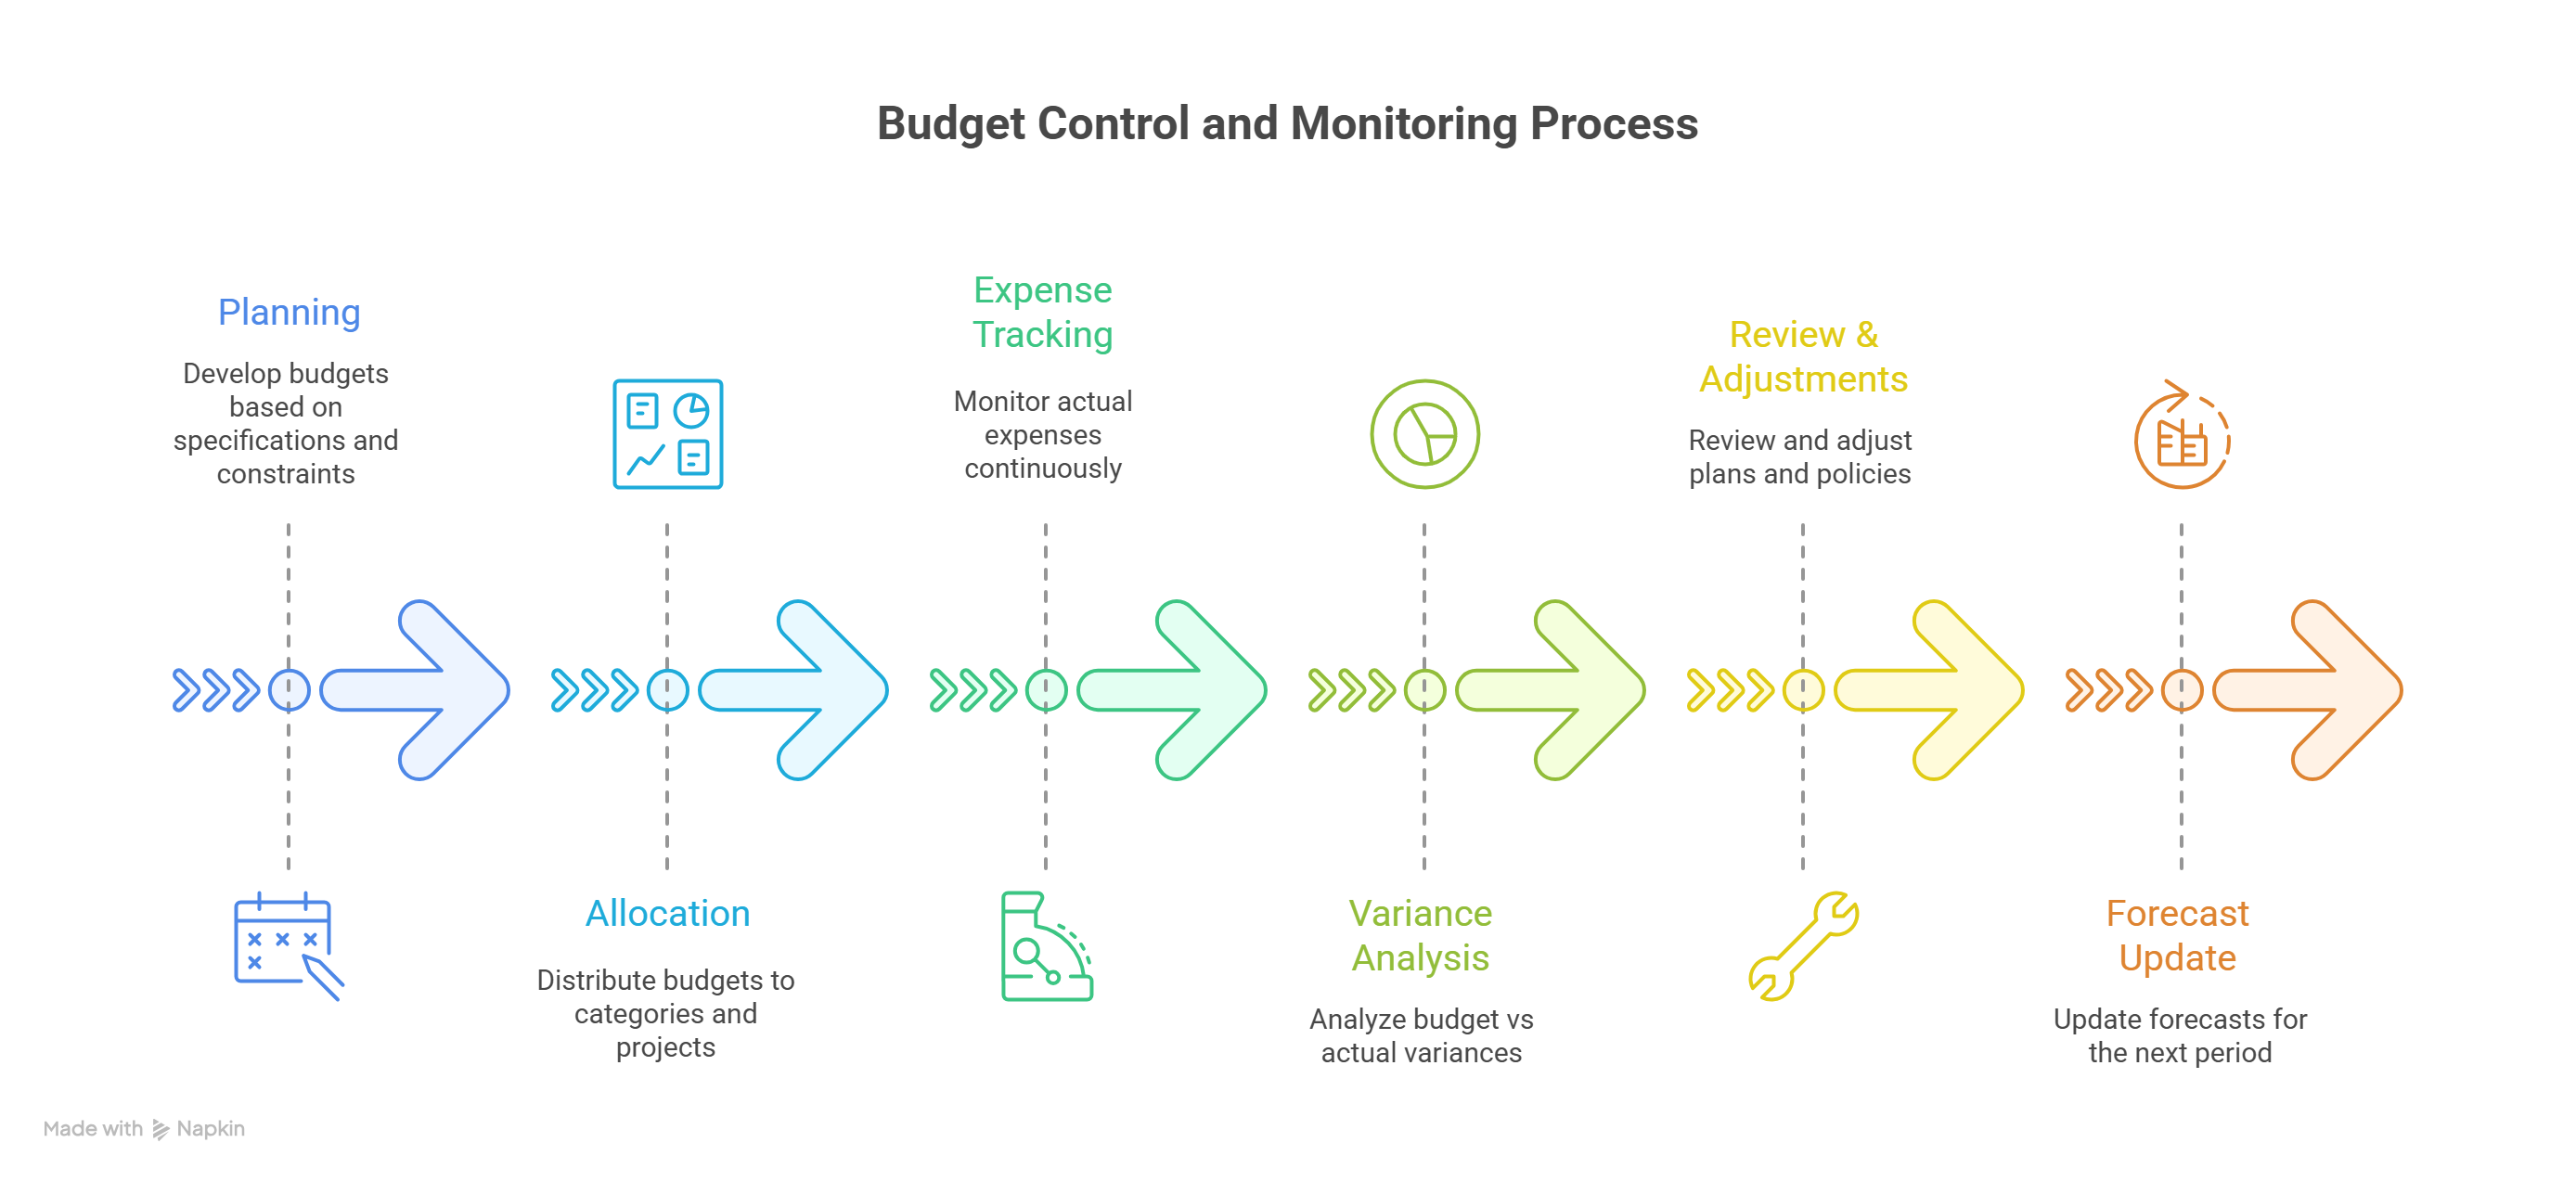
\includegraphics[width=0.9\textwidth]{assets/images/budget_control.png}
    \caption{Budget Control and Monitoring Process}
    \label{fig:budget_control}
\end{figure}

Figure \ref{fig:budget_control} demonstrates the comprehensive budget control and monitoring process, showing the continuous cycle from budget planning through expense monitoring, variance analysis, and performance evaluation. The diagram illustrates the key performance indicators and control mechanisms that ensure effective budget management throughout the project lifecycle.

\subsection{Expense Monitoring and Tracking}
The expense monitoring and tracking system is designed to provide real-time visibility into project expenditures and ensure that all expenses are properly recorded and controlled. This system includes regular monitoring of actual expenses against budgeted amounts, tracking of expense trends, and identification of potential budget overruns or variances.

The expense monitoring process involves regular reviews of financial reports, analysis of expense patterns, and identification of areas where costs may be exceeding budgeted amounts. The tracking system provides detailed information about each expense, including the date, amount, category, and approval status. This information is used to identify trends and make informed decisions about budget management.

The expense monitoring and tracking system is designed to provide early warning of potential budget issues and enable proactive management of project finances. This approach helps to ensure that projects remain within budget and that any necessary adjustments can be made in a timely manner.

\subsection{Variance Analysis and Reporting}
Variance analysis is conducted regularly to identify and analyze differences between budgeted and actual expenses. This analysis helps to identify the causes of variances and determine whether corrective action is needed. The variance analysis process includes both quantitative analysis of expense differences and qualitative analysis of the factors that may have contributed to these variances.

The variance reporting process involves preparing detailed reports that explain the causes of variances and recommend corrective actions. These reports are distributed to relevant stakeholders and are used to inform decision-making about budget adjustments and project management strategies. The variance analysis and reporting process helps to ensure that budget issues are identified and addressed in a timely manner.

The variance analysis and reporting system is designed to provide comprehensive information about budget performance and enable informed decision-making about project finances. This approach helps to ensure that projects remain financially viable and that any necessary adjustments can be made based on accurate and timely information.

\subsection{Cost Control Procedures}
Cost control procedures are implemented throughout the project lifecycle to ensure that expenses are kept within budget and that resources are used efficiently. These procedures include regular reviews of expense authorizations, monitoring of procurement activities, and analysis of cost trends. The cost control procedures are designed to prevent unnecessary expenses and ensure that all expenditures are properly justified and authorized.

The cost control process includes regular reviews of project expenses, analysis of cost trends, and identification of opportunities for cost savings. This process involves input from various departments and stakeholders to ensure that cost control measures are effective and do not compromise project quality or safety. The cost control procedures are regularly reviewed and updated to reflect changing project needs and market conditions.

The cost control procedures are designed to be proactive and preventive, helping to identify potential cost issues before they become significant problems. This approach helps to ensure that projects remain within budget while maintaining quality and safety standards.

\subsection{Budget Revision and Adjustment}
The budget revision and adjustment process allows for changes to project budgets when necessary due to changing project requirements, market conditions, or other factors. This process involves careful analysis of the reasons for budget changes and ensures that all adjustments are properly documented and authorized. The budget revision process includes input from various stakeholders and requires approval at the appropriate level of management.

The budget adjustment process is designed to be flexible and responsive to changing project needs while maintaining overall financial control. This process includes regular reviews of budget performance and identification of areas where adjustments may be needed. The budget revision and adjustment process helps to ensure that projects remain financially viable and that resources are allocated efficiently.

The budget revision and adjustment process is designed to ensure that all budget changes are properly justified and authorized. This approach helps to maintain financial control while allowing for necessary adjustments to project budgets.

\subsection{Financial Performance Metrics}
Financial performance metrics are used to evaluate the effectiveness of budget management and financial control procedures. These metrics include measures such as budget variance percentages, cost efficiency ratios, and financial performance indicators. The financial performance metrics are regularly reviewed and analyzed to identify trends and areas for improvement.

The financial performance metrics are designed to provide comprehensive information about project financial performance and enable informed decision-making about budget management strategies. These metrics help to identify areas where financial performance can be improved and provide the basis for developing more effective budget management procedures.

The financial performance metrics system is designed to provide timely and accurate information about project financial performance. This approach helps to ensure that budget management decisions are based on accurate and relevant information.
